\documentclass[UTF8,11pt]{ctexart}
\usepackage[a4paper,margin=22mm]{geometry}
\usepackage{graphicx,enumitem,amssymb,tabularx}
\usepackage[normalem]{ulem}
\usepackage{xeCJKfntef}
\setlength{\parindent}{0pt}
\setlength{\parskip}{.6em}
\sloppy
\begin{document}
\section*{2021年6月英语六级真题(第1套)}
\subsection*{\textbf{2021}年\textbf{6}月大学英语六级考试真题(一)}


\subsection*{\textbf{Part I} \textbf{Writing} \textbf{(30 minutes)}}


\textbf{Directions: }\textbf{\textit{For this part, you are allowed 30 minutes to write an essay based on the graph below. You}} \textbf{\textit{should start your essay with a brief description of the graph and comment on China's achievements in}} \textbf{\textit{urbanization. You should write at least 150 words but no more than200 words.}} \textbf{Degree of urbanization in China from 1980 to 2019}


\begin{center}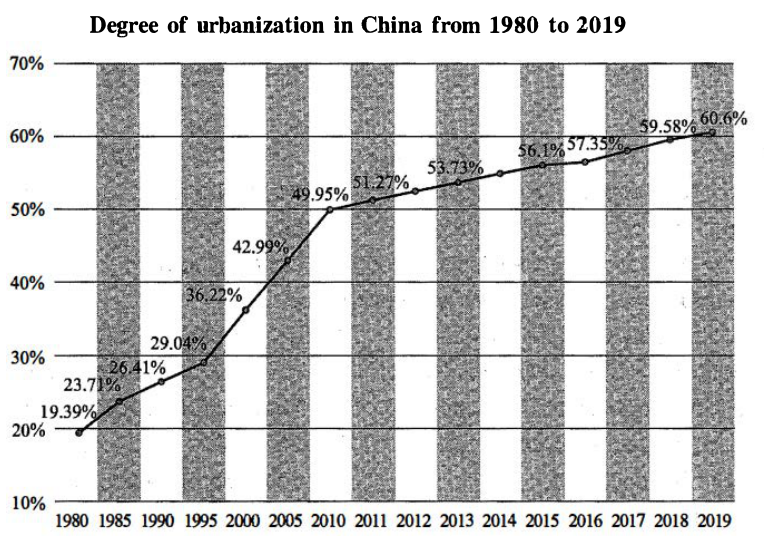
\includegraphics[width=.85\linewidth,height=.55\textheight,keepaspectratio]{2021-06-01.assets/figure-001-003.png}\end{center}

\subsection*{\textbf{Part n:} \textbf{Listening Comprehension} \textbf{( 30 minutes)}}


\subsection*{\textbf{Section A}}


\textbf{Directions: }\textbf{\textit{In this section, you will hear two long conversations. At the end of each conversation, you will}} \textbf{\textit{hear four questions. Both the conversation and the questions will be spoken only once. After you hear a}} \textbf{\textit{question, you must choose the best (Jnswer from the four choices marked A), B), }}C) \textbf{\textit{and }}D). \textbf{\textit{Then mark}} \textbf{\textit{the corresponding letter on Answer Sheet 1 with a single line through the centre.}}


\textbf{Questions 1 to 4 are based on the conversation you have just heard.}


1.


\begin{itemize}[leftmargin=2em,itemsep=.2em,topsep=.4em]\item[A.] He is going to leave his present job.
\item[B.] He is going to attend a job interview.
\item[C.] He will meet his new manager in two weeks.
\item[D.] He will tell the management how he really feels.
\end{itemize}

2.


\begin{itemize}[leftmargin=2em,itemsep=.2em,topsep=.4em]\item[A.] \textbf{It }should be carefully analyzed.
\item[B.] \textbf{It }should be kept private.
\item[C.] It can be quite useful to senior managers.
\item[D.] It can improve interviewees' job prospects.
\end{itemize}

3.


\begin{itemize}[leftmargin=2em,itemsep=.2em,topsep=.4em]\item[A.] \textbf{It }may do harm to his fellow employees.
\item[B.] \textbf{It }may displease his immediate .superiors.
\item[C.] It may adversely affect his future career prospects.
\item[D.] \textbf{It }may leave a negative impression on the interviewer.
\end{itemize}

4.


\begin{itemize}[leftmargin=2em,itemsep=.2em,topsep=.4em]\item[A.] Pour out his frustrations on a rate-your-employer website.
\item[B.] Network with his close friends to find a better employer.
\item[C.] Do some practice for the exit interview.
\item[D.] Prepare a comprehensive exit report.
\end{itemize}

\textbf{Questions 5 to 8 are based on the conversation you have just heard.}


5.


\begin{itemize}[leftmargin=2em,itemsep=.2em,topsep=.4em]\item[A.] Her career as a botanist.
\item[B.] Her latest documentary.
\item[C.] Her month-long expedition.
\item[D.] Her unsuccessful journey.
\end{itemize}

6.


\begin{itemize}[leftmargin=2em,itemsep=.2em,topsep=.4em]\item[A.] She was caught in a hurricane.
\item[B.] She had to live like a vegetarian.
\item[C.] She suffered from water shortage.
\item[D.] She had to endure many hardships.
\end{itemize}

7.


\begin{itemize}[leftmargin=2em,itemsep=.2em,topsep=.4em]\item[A.] They could no longer bear the humidity.
\item[B.] They had no more food in the canoe.
\item[C.] A flood was approaching.
\item[D.] A hurricane was coming.
\end{itemize}

\noindent\begin{tabularx}{\linewidth}{@{}lXXXX@{}}8. & \textbf{A.} It was memorable. & \textbf{B.} It was unbearable. & \textbf{C.} It was fruitful. & \textbf{D.} It was uneventful.\\\end{tabularx}\par

'.


\subsection*{\textbf{Section B}}


\textbf{Directions: }\textit{In this section, you will hear two passages. At the end of each passage }, \textit{you will hear three or} \textit{four questions. Both the passage and the questions will be spoken only once. After you hear a question }, \textit{you} \textit{must choose the best answer from the four choices marked }A), B), C) \textit{and }D). \textit{Then mark the} \textit{corresponding letter on }\textbf{\textit{Answer Sheet 1 }}\textit{with a single line through the centre.}


\textbf{Questions 9 to 11 are based on the passage you have just heard.}


9.


\begin{itemize}[leftmargin=2em,itemsep=.2em,topsep=.4em]\item[A.] It ensures the accuracy of their arguments.
\item[B.] It diminishes laymen's interest in science.
\item[C.] It hurts laymen's dignity and self-esteem.
\item[D.] It makes their expressions more explicit.
\end{itemize}

10.


\begin{itemize}[leftmargin=2em,itemsep=.2em,topsep=.4em]\item[A.] They will see the complexity of science.
\item[B.] They feel great respect towards scientists.
\item[C.] They tend to disbelieve the actual science.
\item[D.] They can learn to communicate with scientists.
\end{itemize}

11.


\begin{itemize}[leftmargin=2em,itemsep=.2em,topsep=.4em]\item[A.] Explain all the jargon terms.
\item[B.] Do away with jargon terms.
\item[C.] Find appropriate topics.
\item[D.] Stimulate their interest.
\end{itemize}

\textbf{Questions 12 to 15 are based on the passage you have just heard.}


12.


\begin{itemize}[leftmargin=2em,itemsep=.2em,topsep=.4em]\item[A.] There were oil deposits below a local gassy hill.
\item[B.] The erupting gas might endanger local children.
\item[C.] There was oiHeakage-along the Gulf Coast.
\item[D.] The local gassy hill might start a huge fire.
\end{itemize}

13.


\begin{itemize}[leftmargin=2em,itemsep=.2em,topsep=.4em]\item[A.] The massive gas underground.
\item[B.] Their lack of the needed skill.
\item[C.] Their lack of suitable tools.
\item[D.] The sand under the hill.
\end{itemize}

14.


\begin{itemize}[leftmargin=2em,itemsep=.2em,topsep=.4em]\item[A.] It was not as effective as he claimed.
\item[B.] It rendered many oil workers jobless.
\item[C.] It gave birth to the oil drilling industry.
\item[D.] It was not popularized until years later.
\end{itemize}

15.


\begin{itemize}[leftmargin=2em,itemsep=.2em,topsep=.4em]\item[A.] It ruined the state's cotton and beef industries.
\item[B.] It totally destroyed the state's rural landscape.
\item[C.] It resulted in an oil surplus all over the world.
\item[D.] It radically transformed the state's economy.
\end{itemize}

\subsection*{\textbf{Section C}}


\textbf{Directions: }\textit{In this section }, \textit{you will hear three recordings of lectures or talks followed by three or four} \textit{questions. The recordings will be played only once }. \textit{After you hear a question }, \textit{you must choose the best} \textit{answer from the four choices marked }A), B), C) \textit{and }D). \textit{Then mark the corresponding letter on }\textbf{\textit{Answer}} \textbf{\textit{Sheet 1 }}\textit{with a single line through the centre.}


\textbf{Questions 16 to 18 are based on the recording you have just heard.}


\noindent\begin{tabularx}{\linewidth}{@{}lXXXX@{}}16. & \textbf{A.} Insufficient motivation. & \textbf{B.} Tough regulations. & \textbf{C.} Unsuitable jobs. & \textbf{D.} Bad managers.\\\end{tabularx}\par

\noindent\begin{tabularx}{\linewidth}{@{}lXXXX@{}}17. & \textbf{A.} Ineffective training. & \textbf{B.} Toxic company culture. & \textbf{C.} Overburdening of managers. & \textbf{D.} Lack of regular evaluation.\\\end{tabularx}\par

18.


\begin{itemize}[leftmargin=2em,itemsep=.2em,topsep=.4em]\item[A.] \textbf{It }was based only on the perspective of employees.
\item[B.] \textbf{It }provided meaningful clues to solving the problem.
\item[C.] \textbf{It }was conducted from frontline managers' point of view.
\item[D.] \textbf{It }collected feedback from both employers and employees.
\end{itemize}

\textbf{Questions 19 to 21 are based on the recording you have just heard.}


19.


\begin{itemize}[leftmargin=2em,itemsep=.2em,topsep=.4em]\item[A.] \textbf{It }is expanding at an accelerating speed.
\item[B.] \textbf{It }is bringing prosperity to the region.
\item[C.] It is yielding an unprecedented profit.
\item[D.] \textbf{It }is seeing an automation revolution.
\end{itemize}

20.


\begin{itemize}[leftmargin=2em,itemsep=.2em,topsep=.4em]\item[A.] \textbf{It }creates a lot of new jobs.
\item[B.] \textbf{It }exhausts res<;mrces sooner.
\item[C.] \textbf{It }causes conflicts between employers and employees.
\item[D.] \textbf{It }calls for the retraining of unskilled mining workers.
\end{itemize}

21.


\begin{itemize}[leftmargin=2em,itemsep=.2em,topsep=.4em]\item[A.] They will wait to see its effect.
\item[B.] They welcome it with open arms.
\item[C.] They accept it with reservations.
\item[D.] They are strongly opposed to it.
\end{itemize}

\textbf{Questions 22 to 25 are based on the recording you have just heard.}


22.


\begin{itemize}[leftmargin=2em,itemsep=.2em,topsep=.4em]\item[A.] They have experienced a gradual decline since the year of 2017.
\item[B.] Their annual death rate is about twice that of the global average.
\item[C.] They kill more people than any infectious disease.
\item[D.] Their cost to the nation's economy is incalculable.
\end{itemize}

23.


\begin{itemize}[leftmargin=2em,itemsep=.2em,topsep=.4em]\item[A.] They are not as reliable as claimed.
\item[B.] They rise and fall from year to year.
\item[C.] They don't reflect the changes in individual countries.
\item[D.] They show a difference between rich and poor nations.
\end{itemize}

24.


\begin{itemize}[leftmargin=2em,itemsep=.2em,topsep=.4em]\item[A.] Many of them are investing heavily in infrastructure.
\item[B.] Many of them have seen a decline in road-death rates.
\item[C.] Many of them are following the example set by Thailand.
\item[D.] Many of them have increasing numbers of cars on the road.
\end{itemize}

25.


\begin{itemize}[leftmargin=2em,itemsep=.2em,topsep=.4em]\item[A.] Foster better driving behavior.
\item[B.] Abolish all outdated traffic rules.
\item[C.] Provide better training for drivers.
\item[D.] Impose heavier penalties on speeding.
\end{itemize}

\textbf{Part JI[} \textbf{Reading Comprehension} \textbf{( 40 minutes)}


\subsection*{\textbf{Section A}}


\noindent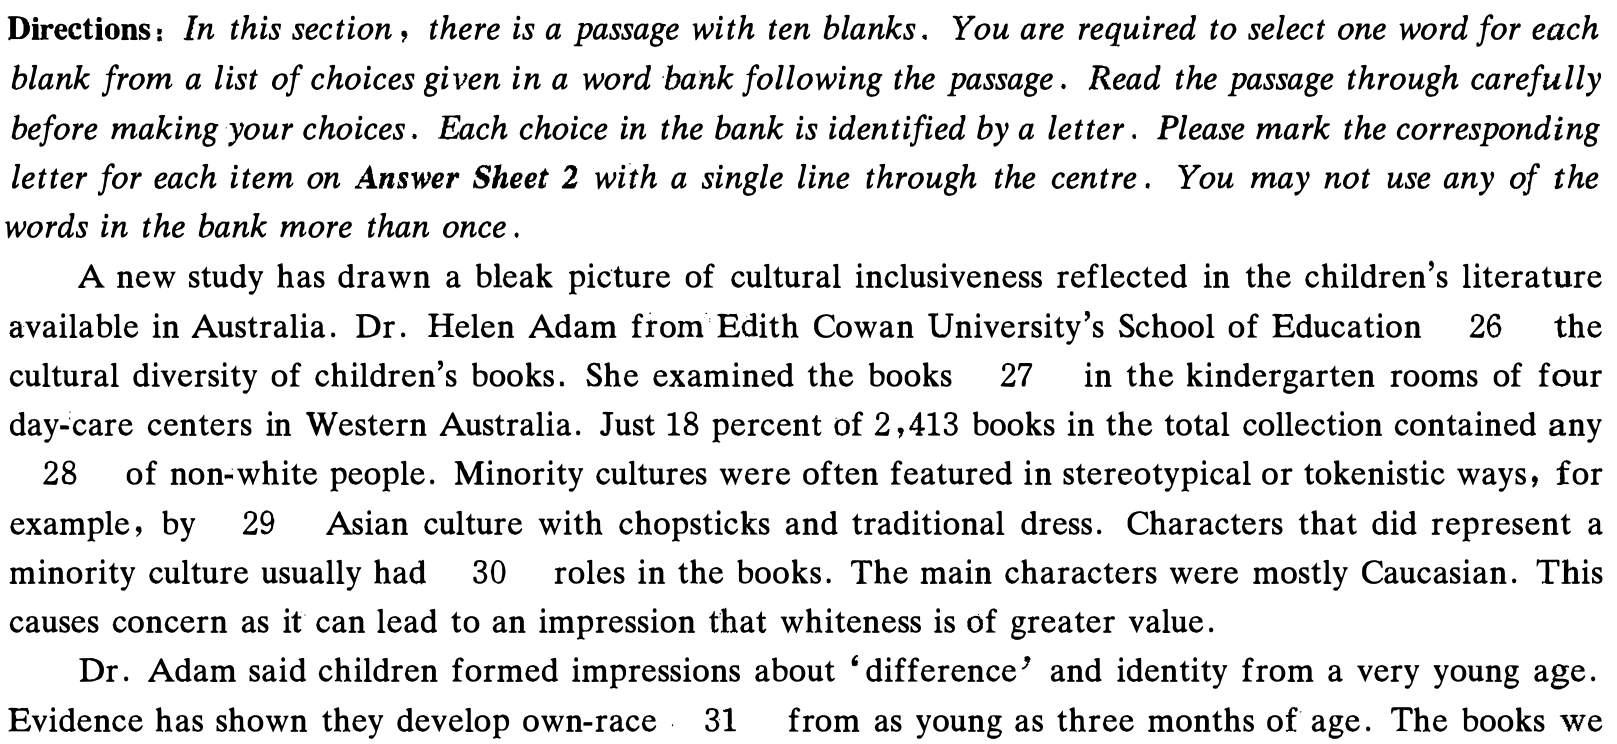
\includegraphics[width=\linewidth,height=.8\textheight,keepaspectratio]{2021-06-01.assets/char-003-line-020.png}\par

\noindent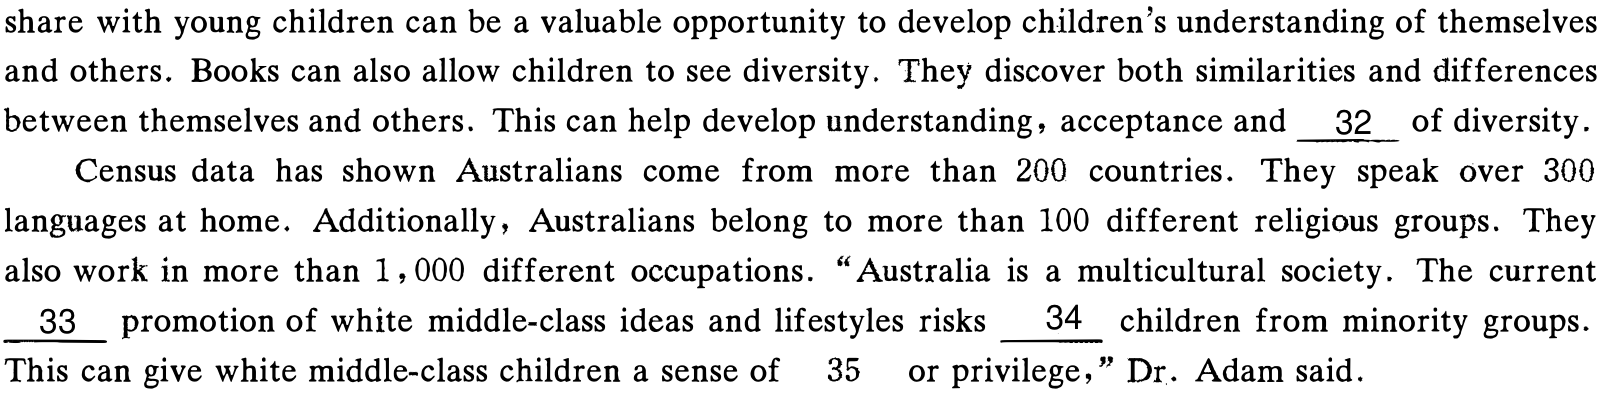
\includegraphics[width=\linewidth,height=.8\textheight,keepaspectratio]{2021-06-01.assets/char-004-line-000.png}\par

\begin{itemize}[leftmargin=2em,itemsep=.2em,topsep=.4em]\item[A.] alienating
\item[B.] appreciation
\item[C.] bias
\item[D.] fraud
\item[E.] housed \textperiodcentered{}
\item[F.] investigated
\item[G.] overwhelming
\item[H.] portraying
\item[I.] representation
\item[J.] safeguarded 0) threshold
\item[K.] ' secondarysecondary
\item[L.] superiority
\item[M.] temperament
\item[N.] tentative
\end{itemize}

\subsection*{\textbf{Section B}}


\textbf{Directions: }\textbf{\textit{In this section, you are going to read a passage with ten statements attached to it. Each}} \textbf{\textit{statement contains information given in one of the paragraphs. Identify the paragraph from which the}} \textbf{\textit{information is derived. You may choose a paragraph more than once. Each paragraph is marked with a}} \textbf{\textit{letter }}. \textbf{\textit{Answer the questions by marking the corresponding letter on Answer Sheet }}\textbf{2} . \textbf{How Marconi Gave Us the Wireless World}


A) A hundred years before iconic figures like Bill Gates and Steve Jobs permeated our lives, an Irish- Italian inventor laid the foundation of the communication explosion of the 21st century. Guglielmo Marconi was arguably the first truly global figure in modern communication. Not only was he the first to communicate globally, he was the first to think globally about communication. Marconi may not have been the greatest inventor of his time, but more than anyone else, he brought about a fundamental shift in the way we communicate.


B) Today's globally networked media and conimunication system has its origins in the 19th century, when, for the first time, messages were sent electronically across great distances. The telegraph, the -telephone, and radio were the obvious predecessors of the-Internet, -iPotls, and-mobile phones. What made the link from then to now was the development of wireless communication. Marconi was the first to develop and perfect this system, using the recently-discovered "air waves" that make up the electromagnetic spectrum.


C) Between 1896, when he applied for his first patent in England at the age of 22, and his death in Italy in 1937, Marconi was at the center of every major innovation in electronic communication. He was also a skilled and sophisticated organizer, an entrepreneurial innovator, who mastered the use of corporate strategy, media relations, government lobbying, international diplomacy, patents, and prosecution. Marconi was really interested in only one thing: the extension of mobile, personal, long- distance communication to the ends of the earth ( and beyond, if we can believe some reports) . Some like to refer to him as a genius, but if there was any genius to Marconi it was this vision.


D) In 1901 he succeeded in signaling across the Atlantic, from the west coast of England to Newfoundland in the USA, despite the claims of science that it could not be done. In 1924 he convinced the British government to encircle the world with a chain of wireless stations using the latest technology that he had devised, shortwave radio. There are some who say Marconi lost his edge when commercial broadcasting came along; he didn't see that radio could or should be used to \textbf{\textit{frivolous }}(::JGJMJ(ID) ends. In one of his last public speeches, a radio broadcast to the United States in March 1937, he deplored that broadcasting had become a one-way means of communication and foresaw it moving in another


\noindent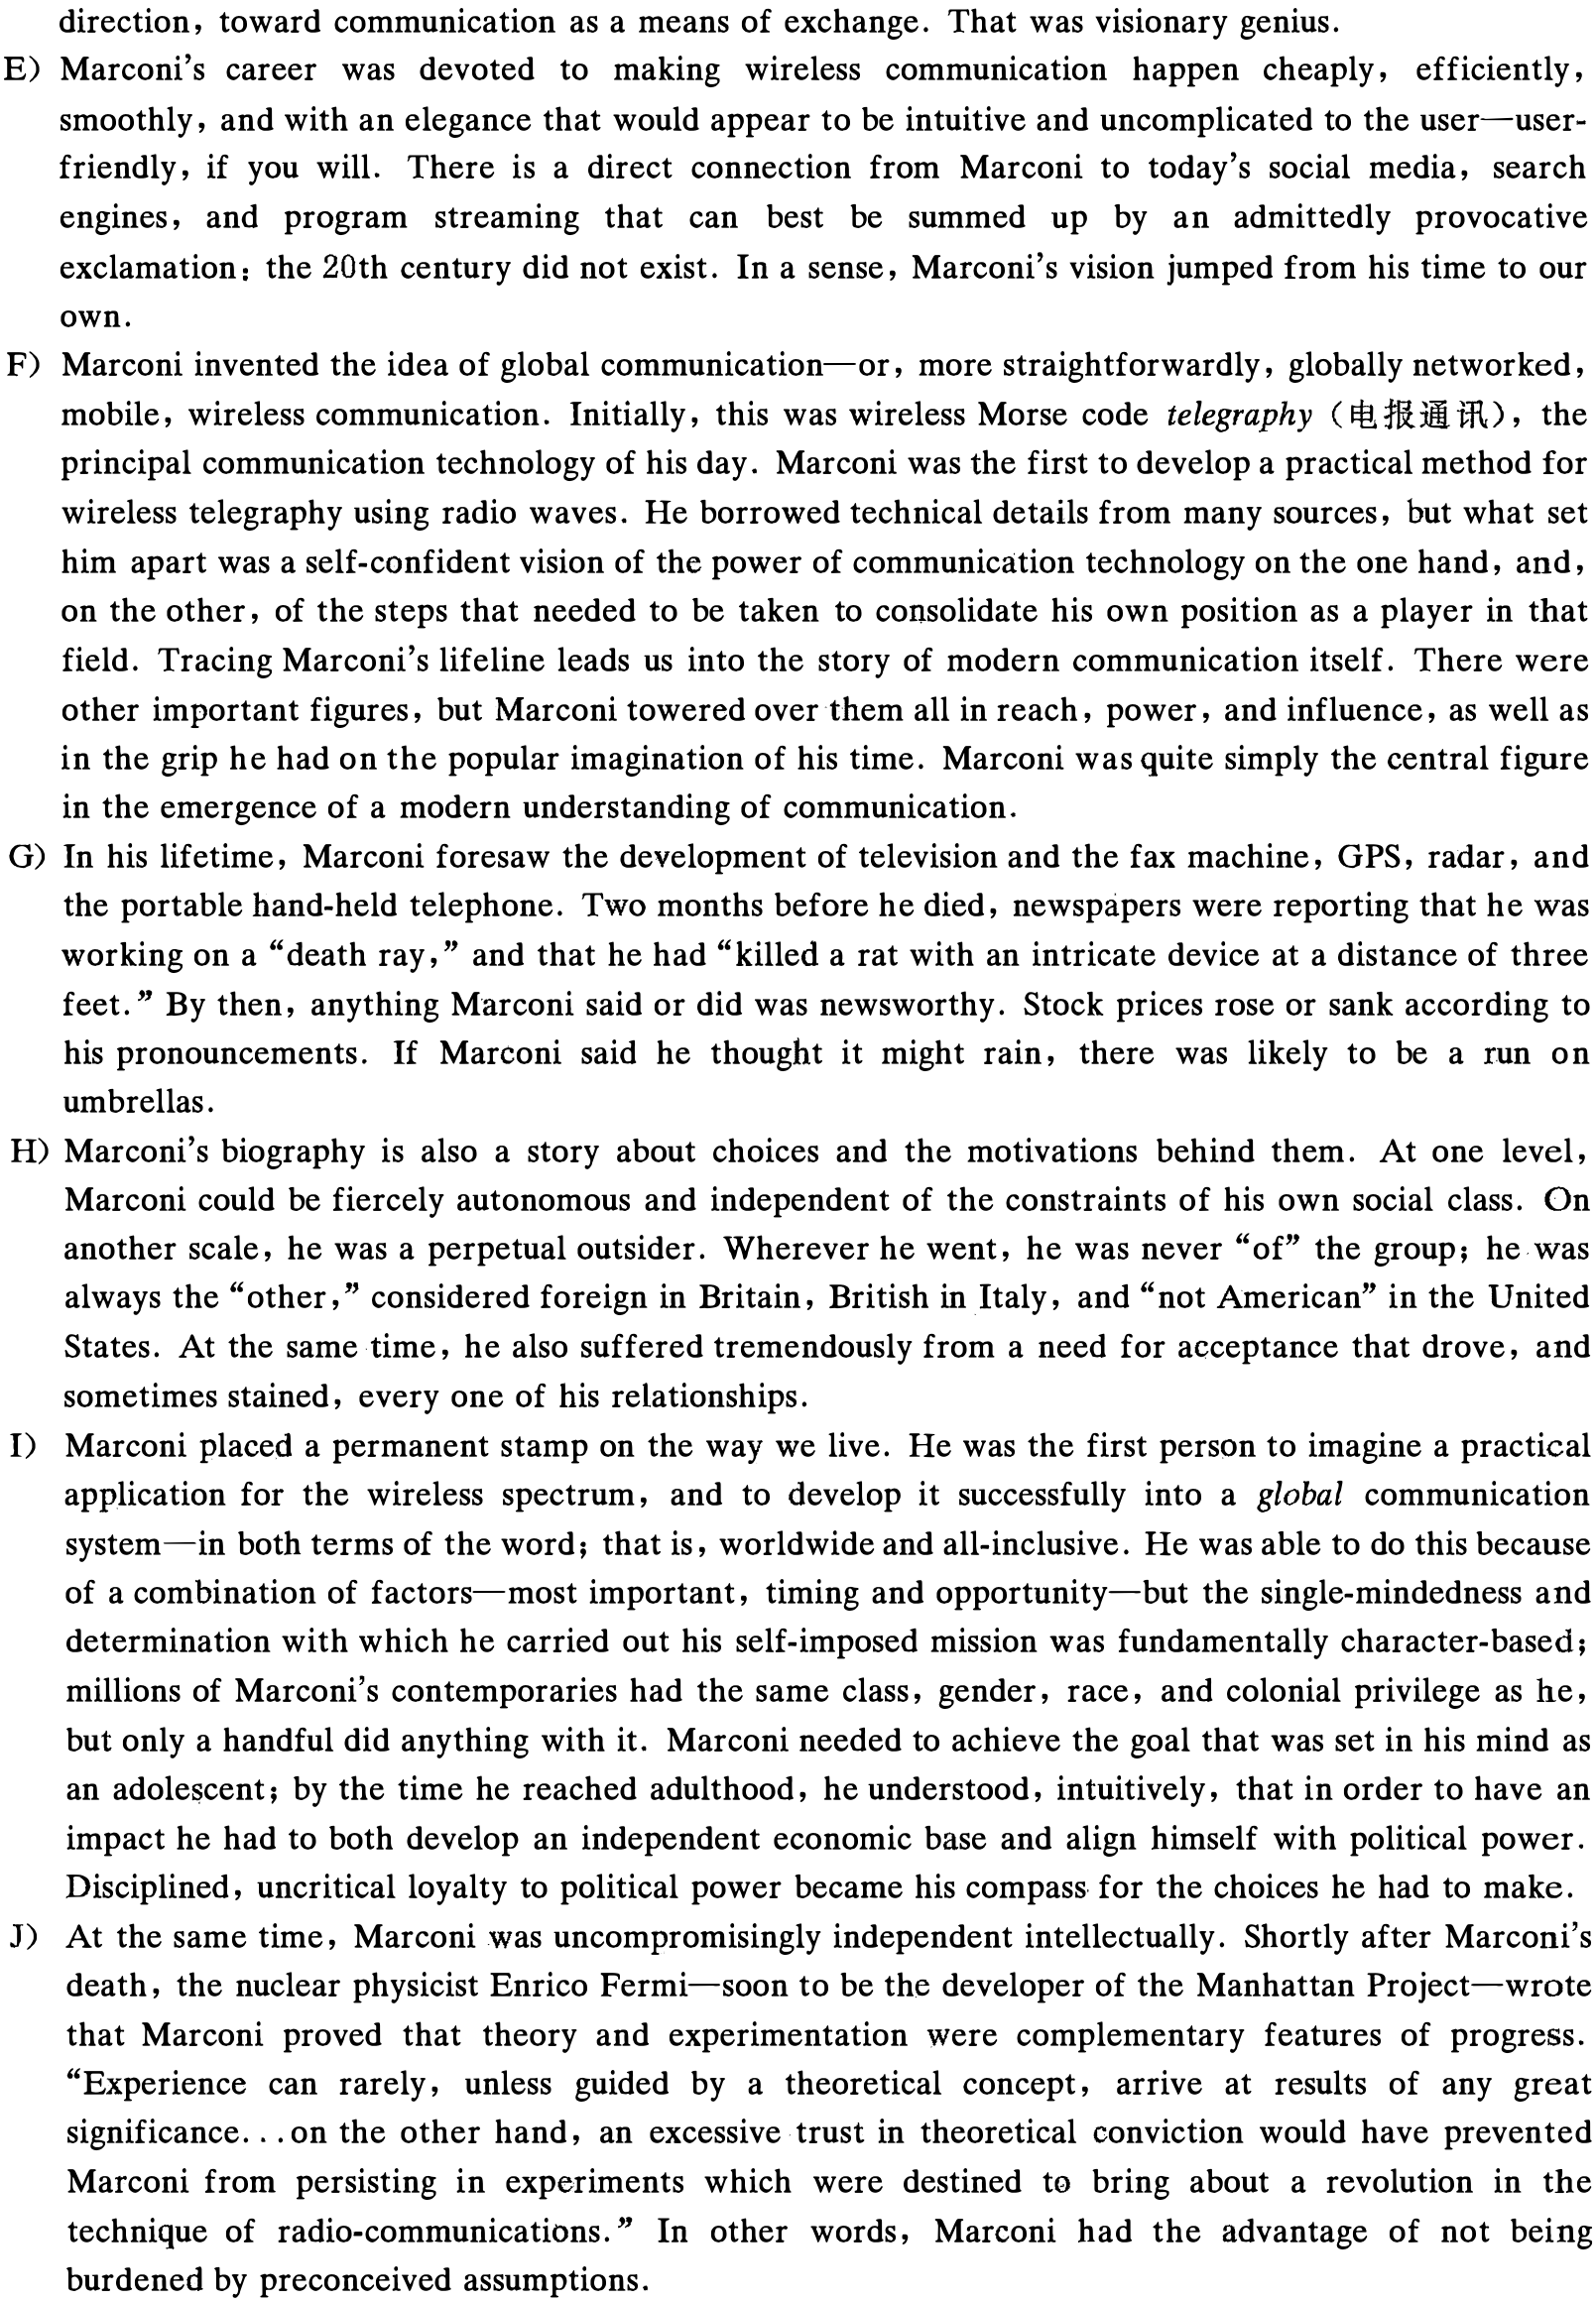
\includegraphics[width=\linewidth,height=.8\textheight,keepaspectratio]{2021-06-01.assets/char-005-line-000.png}\par

K) The most controversial aspect of Marconi's life-and the reason why there has been no satisfying biography of Marconi until now-was his uncritical embrace of Benito Mussolini. At first this was not problematic for him. But as the \textit{regressive }( fftliJH1g) nature of Mussolini's \textperiodcentered{}regime became clear, he began to suffer a crisis of conscience. However, after a lifetime of moving within the circles of power, he was unable to break with authority, and served Mussolini faithfully ( as president of Italy's national research council and royal academy, as well as a member of the Fascist Grand Council) until the day he died-conveniently-in 1937, shortly before he would have had to take a stand in the conflict that consumed a world that he had, in part, created.


36. Marconi was central to our present-day understanding of communication.


37. As an adult, Marconi had an intuition that he had to be loyal to politicians in order to be influential.


38. Marconi disapproved of the use of wireless communication for commercial broadcasting.


39. Marconi's example demonstrates that theoretical concepts and experiments complement each other in


making progress in science and technology.


40. Marconi's real interest lay in the development of worldwide wireless communication:


41. Marconi spent his whole life making wireless communication simple to use.


42. Because of his long-time connection with people in power, Marconi was unable to cut himself off from


the fascist regime in Italy.


43. In his later years, Marconi exerted a tremendous influence on all aspects of people's life.


44. What connected the 19th century and our present time was the development of wireless


communication.


45. Despite his autonomy, Marconi felt alienated and suffered from a lack of acceptance.


\subsection*{\textbf{Section C}}


\textbf{Directions: }\textit{There are 2 passages in this section. Each passage is followed by some questions or unfinished} \textit{statements. For each of them there are four choices marked A), }B), C) \textit{and }D). \textit{You should decide on the} \textit{best choice and mark the corresponding letter on }\textbf{\textit{Answer Sheet }}2 \textit{with a single line through the centre.}


\subsection*{\textbf{Passage One}}


\textbf{Questions 46 to 50 are based on the following passage.}


Humans are fascinated by the source of their failings and virtues. This preoccupation inevitably leads to an old debate: whether nature or nurture moulds us more. A revolution in genetics has poised this as a modern political question about the character of our society: personalities are hard-wired into our genes what can governments do to help us? It feels morally questionable, yet claims of genetic selection by intelligence are making headlines. This is down to “hereditarian” (遗传论的) science and a recent paper claimed “udifferences in exam performance between pupils attending selective and non-selective schools mirror the genetic differences between them”. With such an assertion, the work was predictably greeted by a lot of absurd claims about “genetics determining academic success”. What the research revealed was the rather less surprising result: the educational benefits of selective schools largely disappear once pupils' inborn ability and socio-economic background were taken into account. It is a glimpse of the blindingly obvious-and there's nothing to back strongly either a hereditary or environmental argument. Yet the paper does say children are “unintentionally genetically selected” by the school system. Central to hereditarian science is a tall claim: that identifiable variations in genetic sequences can predict an individual's aptness to learn, reason and solve problems. This is problematic on many levels. A teacher could not seriously tell a parent their child has a low genetic tendency to study when external factors clearly exist. Unlike-minded academics say the inheritability of human traits is scientifically unsound. At best there is a weak statistical association and not a causal link between DNA and intelligence. Yet sophisticated statistics are used to create an intimidatory atmosphere of scientific certainty. While there's an undoubted genetic basis to individual difference, it is wrong to think that socially


defined groups can be genetically accounted for. The fixation on genes as destiny is surely false too. Medical predictability can rarely be based on DNA alone; the environment matters too. Something as complex as intellect is likely to be affected by many factors beyond genes. If hereditarians want to advance their cause it will require more balanced interpretation and not just acts. of advocacy.


Genetic selection is a way of exerting influence over others, "the ultimate collective control of human destinies," as writer H. G. Wells put it. Knowledge becomes power and power requires a sense of responsibility. In understanding cognitive ability, we must not elevate discrimination to a science; allowing people to climb the ladder of life only as far as their cells might suggest. This will need a more sceptical eye on the science. As technology progresses, we all have a duty to make sure that we shape a future that we would want to find ourselves in.


46. What did a recent research paper claim?


\begin{itemize}[leftmargin=2em,itemsep=.2em,topsep=.4em]\item[A.] The type of school students attend makes a difference to their future.
\item[B.] Genetic differences between students are far greater than supposed.
\item[C.] The advantages of selective schools are too obvious to ignore.
\item[D.] Students' academic performance is determined by their genes.
\end{itemize}

47. What does the author think of the recent research?


\begin{itemize}[leftmargin=2em,itemsep=.2em,topsep=.4em]\item[A.] Its result was questionable.
\item[B.] Its implication was positive.
\item[C.] Its influence was rather negligible.
\item[D.] Its conclusions were enlightening.
\end{itemize}

48. What does the author say about the relationship between DNA and intelligence?


\begin{itemize}[leftmargin=2em,itemsep=.2em,topsep=.4em]\item[A.] It is one of scientific certainty.
\item[B.] It is not one of cause and effect.
\item[C.] It is subject to interpretation of statistics.
\item[D.] It is not fully examined by gene scientists.
\end{itemize}

49. What do hereditarians need to do to make their claims convincing?


\begin{itemize}[leftmargin=2em,itemsep=.2em,topsep=.4em]\item[A.] Take all relevant factors into account in interpreting their data.
\item[B.] Conduct their research using more sophisticated technology.
\item[C.] Gather gene data from people of all social classes.
\item[D.] Cooperate with social scientists in their research.
\end{itemize}

50. What does the author warn against in the passage?


\begin{itemize}[leftmargin=2em,itemsep=.2em,topsep=.4em]\item[A.] Exaggerating the power of technology in shaping the world.
\item[B.] Losing sight of professional ethics in conducting research.
\item[C.] Misunderstanding the findings of human cognition research.
\item[D.] Promoting discrimination in the name of science.
\end{itemize}

\noindent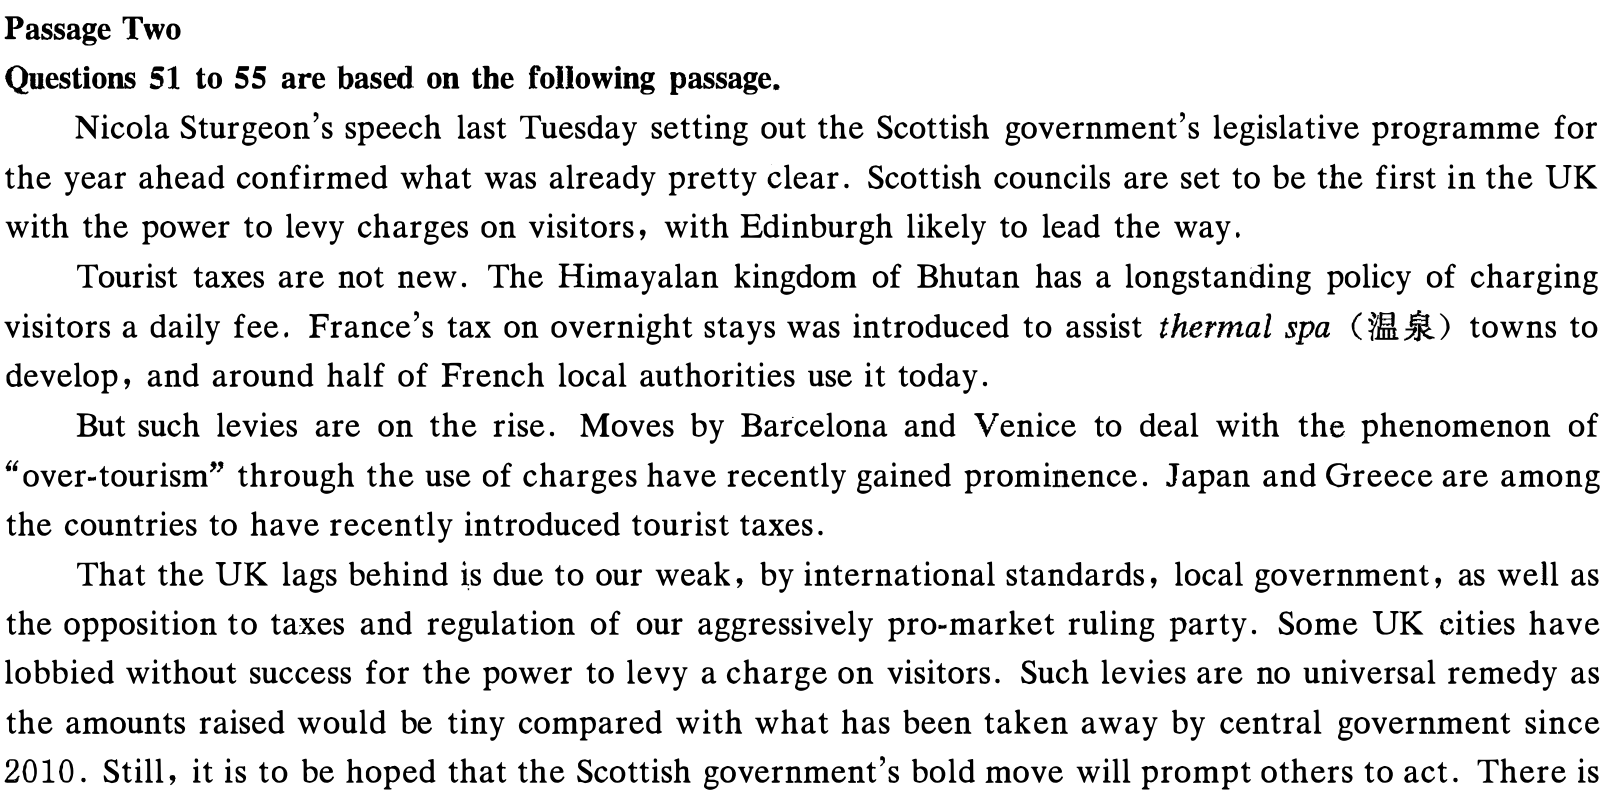
\includegraphics[width=\linewidth,height=.8\textheight,keepaspectratio]{2021-06-01.assets/char-007-line-012.png}\par

no reason why visitors to the UK, or domestic tourists on holiday in hotspots such as Cornwall, should be exempt from taxation-particularly when vital local services including waste collection, park maintenance and arts and culture spending are under unprecedented strain.


On the contrary, compelling tourists to make a financial contribution to the places they visit beyond their personal consumption should be part of a wider cultural shift. Westerners with disposable incomes have often behaved as if they have a right to go wherever they choose with little regard for the consequences. Just as the environmental harm caused by aviation and other transport must come under far greater scrutiny, the social cost of tourism must also be confronted. This includes the impact of short-term lets on housing costs and quality of life for residents. Several European capitals, including Paris and Berlin, are leading a campaign for tougher regulation by the European Union. It also includes the impact of overcrowding, litter and the kinds of behaviour associated with noisy parties.


There is no "one size fits all" solution to this problem. The existence of new revenue streams for some but not all councils is complicated, and businesses are often opposed, fearing higher costs will make them uncompetitive. But those places that want them must be given the chance to make tourist taxes work.


51. What do we learn from Nicola Sturgeon's speech?


\begin{itemize}[leftmargin=2em,itemsep=.2em,topsep=.4em]\item[A.] The UK is set to adjust its policy on taxation.
\item[B.] Tourists will have to pay a tax to visit Scotland.
\item[C.] The UK will take new measures to boost tourism.
\item[D.] Edinburgh contributes most to Scotland's tourism.
\end{itemize}

52. How come the UK has been slow in imposing the tourist tax?


\begin{itemize}[leftmargin=2em,itemsep=.2em,topsep=.4em]\item[A.] Its government wants to attract more tourists.
\item[B.] The tax is unlikely to add much to its revenue.
\item[C.] Its ruling party is opposed to taxes and regulation.
\item[D.] It takes time for local governments to reach consensus.
\end{itemize}

53. Both international and domestic visitors in the UK should pay tourist tax so as to \_\_\_ \_


\begin{itemize}[leftmargin=2em,itemsep=.2em,topsep=.4em]\item[A.] elevate its tourism to international standards
\item[B.] improve the welfare of its maintenance workers
\item[C.] promote its cultural exchange with other nations
\item[D.] ease its financial burden of providing local services
\end{itemize}

54, What does the author sa-y about Western tourists?


\begin{itemize}[leftmargin=2em,itemsep=.2em,topsep=.4em]\item[A.] They don't seem to care about the social cost of tourism.
\item[B.] They don't seem to mind paying for additional services.
\item[C.] They deem travel an important part of their life.
\item[D.] They subject the effects of tourism to scrutiny.
\end{itemize}

55. What are UK people's opinions about the levy of tourist tax?


\begin{itemize}[leftmargin=2em,itemsep=.2em,topsep=.4em]\item[A.] Supportive.
\item[B.] Skeptical.
\item[C.] Divided.
\item[D.] Unclear.
\end{itemize}

\subsection*{\textbf{Part }\textbf{\textit{N}} \textbf{Translation} \textbf{( 30 minutes)}}


\textbf{Directions: }\textit{For this part, you are allowed 30 minutes to translate a passage from Chinese into English. You}


\textit{should write your answer on }\textbf{\textit{Answer Sheet 2 }}.


海南是仅次于台湾的中国第二大岛,是位于中国最南端的省份。海南岛风景秀丽,气候宜人,阳光充足,生物多样,温泉密布,海水清澈,大部分海滩几乎全年都是游泳和日光浴的理想场所,因而被誉为中国的四季花园和度假胜地,每年都吸引了大批中外游客。


海南1988年建省以来,旅游业、服务业、高新技术产业飞速发展,是中国唯一的省级经济特区。在中央政府和全国人民的大力支持下,海南将建成中国最大的自由贸易试验区。

\end{document}